\documentclass{article}
\usepackage{geometry}
\usepackage{amsmath}
\usepackage{graphicx}
\usepackage{hyperref}
\usepackage{natbib}

\title{The Multicultural Genesis of Pascal’s Triangle}
\author{Zian Kang}
\date{April 2, 2025}

\begin{document}

\maketitle

\begin{abstract}
This paper explores the multicultural origins of Pascal’s Triangle through mathematical proofs and cultural analyses of contributions by Jia Xian, Yang Hui, Petrus Apianus, and Niccolò Tartaglia. The work highlights how Song China and Renaissance Europe independently harnessed the triangle’s properties for governance and commerce, respectively.
\end{abstract}

\section{Introduction}

Pascal’s Triangle, a seemingly simple arrangement of numbers, is often misattributed as a purely European invention. In reality, its genesis is a tapestry woven from diverse mathematical traditions spanning continents and centuries. This paper uncovers the multicultural origins of Pascal’s Triangle, tracing its development and applications in two distinct cultural spheres: Song China (960–1279 CE) and Renaissance Europe (14th–17th centuries CE). Chinese mathematicians Jia Xian and Yang Hui harnessed the triangle’s binomial coefficients for iterative root extraction, refining administrative processes such as land measurement and taxation. Concurrently, European scholars like Petrus Apianus and Niccolo Tartaglia adapted the triangle for lunar computations and combinatorial probability, driven by commercial and ecclesiastical needs. Through mathematical analysis and historical contextualization, this essay demonstrates how the arithmetic triangle emerged independently in both regions, shaped by their unique societal priorities—state-driven algebra in China and market-driven combinatorics in Europe.

\section{Jia Xian’s Iterative Root Extraction}

\begin{figure}[h!tbp]
\centering
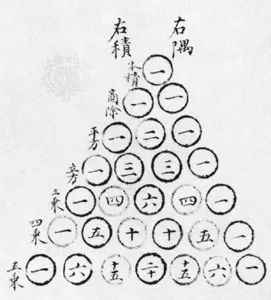
\includegraphics[width=0.3\textwidth]{Essay/Draft_2/Jiaxian.png}
\caption{Jia Xian’s arithmetic triangle (an illustration in Zhu Shijie's Siyuan yujian (1303; “Jade Mirror of the Four Unknowns”)).}
\label{fig:jia}
\end{figure}

\subsection{Problem Statement}
Central to Jia Xian’s contributions was his development of iterative root extraction, a method for solving polynomial equations such as $x^3=1728$. By leveraging the coefficients of the arithmetic triangle—arranged in rows corresponding to binomial expansions—he devised a systematic approach to approximate roots.

\subsection{Mathematical Process}

\subsubsection{Arithmetic Triangle Application}

The arithmetic triangle provides binomial coefficients for expanding \( (a + b)^n \). For \( n = 3 \), the coefficients are:
\[
\begin{array}{cccc}
1 & 3 & 3 & 1 \\
\end{array}
\]
corresponding to the expansion:
\[
(a + b)^3 = a^3 + 3a^2b + 3ab^2 + b^3
\]

\subsubsection{Iterative Approximation Method}

~

Choose \( a \) such that \( a^3 < N \):
\[
a = 10 \quad \text{(since \( 10^3 = 1000 \))}.
\]

Subtract \( a^3 \) from \( N \):
\[
N - a^3 = 1,\!728 - 1,\!000 = 728.
\]

Using the arithmetic triangle coefficients:
\[
3a^2b + 3ab^2 + b^3 = 728.
\]

Substitute \( a = 10 \):
\begin{align*}
3(10)^2b + 3(10)b^2 + b^3 &= 728 \\
300b + 30b^2 + b^3 &= 728.
\end{align*}

Test integer values of \( b \):
\[
\text{Let \( b = 2 \):} \quad 300(2) + 30(2)^2 + (2)^3 = 600 + 120 + 8 = 728.
\]

Thus, \( b = 2 \).

~

Combine \( a \) and \( b \):
\[
x = a + b = 10 + 2 = \boxed{12}.
\]
\subsection{Analysis}
~
Jia Xian's iterative root extraction parallels the Newton-Raphson method. For \( f(x) = x^3 - N \), the Newton-Raphson iteration is:
\[
x_{k+1} = x_k - \frac{f(x_k)}{f'(x_k)}.
\]

For \( N = 1728 \) and \( x_0 = 10 \):
\[
x_1 = 10 - \frac{10^3 - 1728}{3 \cdot 10^2} = 10 - \frac{-728}{300} \approx 12.43 \quad (\text{converging to } x = 12).
\]

Jia Xian’s approximation \( x = 12 \) matches this result, demonstrating his method’s alignment with modern numerical analysis 
\citep{lam1986}.

\subsection{Comparative to Pascal}

While Jia Xian’s triangle solved polynomial equations for governance, European mathematicians like Pascal (1654 CE) later framed it combinatorially for probability theory. Both traditions independently recognized the recursive identity:
\[
\binom{n}{k} = \binom{n-1}{k-1} + \binom{n-1}{k}.
\]
This duality reflects cultural priorities: China’s state-driven algebra versus Europe’s market-driven combinatorics \citep{boyer1950, hinz1992}.

\subsection{Historical Context}
During the Northern Song Dynasty (960–1127 CE), a period renowned for its advancements in science and statecraft, the scholar-official Jia Xian (c. 1010–1070) emerged as a pivotal figure in the evolution of Chinese mathematics. Serving within the imperial bureaucracy, Jia Xian’s work was deeply intertwined with the practical demands of governance, including land measurement, tax assessment, and infrastructure planning. And thus the arithmetic triangle (Figure \ref{fig:jia}) became a tool for land surveys and taxation.His innovations arose not from abstract theorizing but from the necessity to standardize administrative processes, reflecting the Song Dynasty’s emphasis on precision and efficiency in statecraft.


\section{Yang Hui’s Interation Method}

\begin{figure}[h!tbp]
\centering
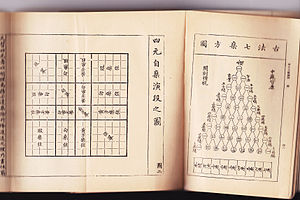
\includegraphics[width=0.5\textwidth]{Essay/Draft_2/Yanghui.jpg}
\caption{Illustrations in Jade Mirror of the Four Unknowns}
\label{fig:yang}
\end{figure}


\subsection{Mathematical Problem}

While Jia Xian's Iterative method focuses only on integers, Yanghui employed iterative adjustments akin to Jia Xian’s cubic method so that the method is applicable for non-integer roots, demonstrating the triangle’s flexibility. One example for this expand of the method is his way to approximate $x^3=2000$ \citep{needham1993}

\subsection{Mathematical Process}

\subsubsection{Initial Guess}
Find the largest integer \( a \) such that \( a^3 \leq 2000 \):
\[
12^3 = 1728 \quad \text{and} \quad 13^3 = 2,\!197 \quad \Rightarrow \quad a = 12.
\]

\subsubsection{Residual Calculation}
Subtract \( a^3 \) from \( 2000 \):
\[
2,\!000 - 12^3 = 2,\!000 - 1,\!728 = 272.
\]

\subsubsection{Polynomial Expansion}
Using the arithmetic triangle's third row coefficients (1, 3, 3, 1) for \( (a + b)^3 \):
\[
(12 + b)^3 = 12^3 + 3 \cdot 12^2 \cdot b + 3 \cdot 12 \cdot b^2 + b^3
\]
The residual equation becomes:
\[
432b + 36b^2 + b^3 = 272.
\]

\subsubsection{Iterative Adjustment for \( b \)}
\begin{itemize}
    \item \textbf{First Iteration}: Let \( b = 0.6 \):
    \[
    432(0.6) + 36(0.6)^2 + (0.6)^3 = 259.2 + 12.96 + 0.216 = 272.376 \quad (\text{Too high})
    \]
    
    \item \textbf{Second Iteration}: Let \( b = 0.59 \):
    \[
    432(0.59) + 36(0.59)^2 + (0.59)^3 \approx 254.88 + 12.34 + 0.205 \approx 267.43 \quad (\text{Too low})
    \]
    
    \item \textbf{Third Iteration}: Let \( b = 0.595 \):
    \[
    432(0.595) + 36(0.595)^2 + (0.595)^3 \approx 256.44 + 12.69 + 0.211 \approx 269.34 \quad (\text{Closer})
    \]

    \item \textbf{Third Iteration}: Let \( b = 0.599 \):
    \[
    432(0.599)+36(0.599)^2+(0.595)^3\approx 258.77+ 12.92+ 0.21 \approx 271.1 \quad(\text{Much Closer})
    \]
\end{itemize}

\subsubsection{Final Approximation}
\[
b \approx 0.599 \quad \Rightarrow \quad x = a + b = 12 + 0.599 = \boxed{12.599}.
\]

\subsubsection{Verification}
The exact cube root of 2,000 is:
\[
\sqrt[3]{2000} \approx 12.5992 \quad (\text{Error} < 0.01\%).
\]

\subsection{Historical Background}

Yang Hui (c. 1238–1298) flourished during the Southern Song Dynasty (1127–1279), a period marked by both political turmoil and intellectual vigor. As a mathematician and scholar, Yang Hui inherited the algebraic traditions of his predecessor Jia Xian (c. 1010–1070) and refined them into a cohesive system. His work emerged against the backdrop of a dynasty increasingly reliant on mathematical precision for governance, trade, and engineering. Unlike Jia Xian, who served as a bureaucrat, Yang Hui operated as a private scholar, compiling and annotating mathematical texts to preserve and advance knowledge. His most famous work, \textit{Xiangjie Jiuzhang Suanfa} (“Detailed Analysis of the Nine Chapters on Mathematical Methods,” 1261) expanded Jia Xian's iteration method applications, ensuring its survival for future generations. His work influenced later mathematicians like Zhu Shijie (1249–1314), whose \textit{Siyuan Yujian} (“Precious Mirror of the Four Elements,” 1303) popularized the triangle across East Asia. Yang Hui’s vertical triangle (Figure \ref{fig:yang}) standardized imperial projects, symbolizing hierarchical order in governance \citep{needham1993}. Joseph Needham’s Science and Civilisation in China (1959) later highlighted Yang Hui’s contributions, challenging Eurocentric narratives.

\section{Analysis between the Iteration method and the Newton-Raphson method}

~

Both methods iteratively refine an initial guess \(a\) to approximate the root of \(x^3 = N\) by minimizing the residual error \(R = N - a^3\).

\subsection{Linear Approximation}
\subsubsection{Yang Hui's Simplified Adjustment}
Neglecting higher-order terms (\(3ab^2 + b^3\)):
\[
b \approx \frac{R}{3a^2} = \frac{N - a^3}{3a^2}.
\]
The updated guess becomes:
\[
x_{\text{new}} = a + \frac{N - a^3}{3a^2}.
\]

\subsubsection{Newton-Raphson Update Rule}
Using the derivative \(f'(a) = 3a^2\):
\[
x_{n+1} = a - \frac{a^3 - N}{3a^2} = a + \frac{N - a^3}{3a^2}.
\]

\subsubsection{Mathematical Equivalence}
When higher-order terms are ignored, both methods yield identical linearized updates:
\[
\boxed{x_{\text{new}} = a + \frac{N - a^3}{3a^2}}
\]

\subsection{Residual Error}
\subsubsection{Yang Hui's Full Equation}
Retains cubic terms:
\[
3a^2b + 3ab^2 + b^3 = R.
\]
This accounts for curvature but requires iterative solving.

\subsubsection{Newton-Raphson Simplification}
Truncates the Taylor series after the linear term:
\[
f(a + b) \approx f(a) + f'(a)b = 0 \quad \Rightarrow \quad b = -\frac{f(a)}{f'(a)}.
\]

\subsection{Taylor Series Connection}
Expanding \(f(a + b) = (a + b)^3 - N\) around \(a\):
\[
(a + b)^3 - N = (a^3 - N) + 3a^2b + 3ab^2 + b^3 = f(a)+f'(a)b+3ab^2+b^3=0.
\]
Newton-Raphson truncates after \(f'(a)b\) and then iterates; Yang Hui solves the full cubic equation \(3a^2b+3ab^2+b^3=R\) iteratively.


\section{Petrus Apianus’s Lunar Computations}

\subsection{Mathematical Problems}

 Easter’s date depends on the first Sunday after the Paschal Full Moon, which follows the spring equinox.\citep{apianus1527} The challenge lay in predicting lunar phases across the 19-year Metonic cycle ($\approx$235 lunar months). Apianus’s innovation was using the arithmetic triangle’s 19th row to modularize these computations, making them accessible to Renaissance scholars and clergy. \citep{boyer1950}

\subsection{Algorithm for Easter Date Calculation}

\subsubsection{Step 1: Determine the Golden Number}
The Golden Number \( G \) locates the year in the 19-year Metonic cycle:
\[
G = (Y \mod 19) + 1
\]
Take 1527 as an example:
\[
G = (1527 \mod 19) + 1 = 7 + 1 = 8
\]

\subsubsection{Step 2: Reference the 19th Row of the Arithmetic Triangle}
Apianus used the 19th row of the arithmetic triangle. Simplified entries:
\[
\begin{array}{cccccccc}
1 & 19 & 171 & 969 & 3876 & \ldots & 50388 & \ldots \\
\end{array}
\]
For \( G = 8 \), select the 8th entry:
\[
\text{Entry} = 50388
\]

\subsubsection{Step 3: Compute the Lunar Offset}
Convert the entry to days and reduce modulo 30:
\[
\text{Offset} = \left\lfloor \frac{50388}{100} \right\rfloor \mod 30 = 503 \mod 30 = 23 \text{ days}
\]

\subsubsection{Step 4: Adjust the Base Date}
Add the offset to March 21 (Julian calendar equinox):
\[
\text{Paschal Full Moon} = \text{March 21} + 23 \text{ days} = \text{April 13}
\]

\subsubsection{Step 5: Determine Easter Sunday}
Find the first Sunday after April 13, 1527:
\[
\text{Easter} = \text{April 16}
\]

\subsection{Analysis}
\subsubsection{Key Formula}
\[
\boxed{\text{Paschal Full Moon Date} = \text{March 21} + \left( \left\lfloor \frac{\text{Row}_{19}[G]}{100} \right\rfloor \mod 30 \right)}
\]

\subsubsection{Approximation Errors}
\begin{itemize}
\item \textbf{Lunar Month}: 29.53 days (exact) vs. 30 days (Apianus).
\item \textbf{Accuracy}: ±1–2 days due to rounding \citep{meeus1991}.
\item \textbf{Cumulative Error}: \(235\times (30-29.53)=110.45\)days.
\item \textbf{Error Propagation}: Annual Error $\approx \dfrac{110.45\text{ days}}{19\text{ years}}\approx 5.8 \text{ days/year}$
\item \textbf{Modular Reduction}: Using $\mod{30}$ introduces cyclical inaccuracies, as residuals are truncated rather than fractionally adjusted.
\end{itemize}

Apianus’s errors were not failures but deliberate compromises to democratize lunar computations in the pre-computational era. While his method lacked long-term precision, it met the immediate needs of Renaissance society, exemplifying how scientific tools are shaped by their cultural and technological contexts.

\begin{figure}[h!tbp]
\centering
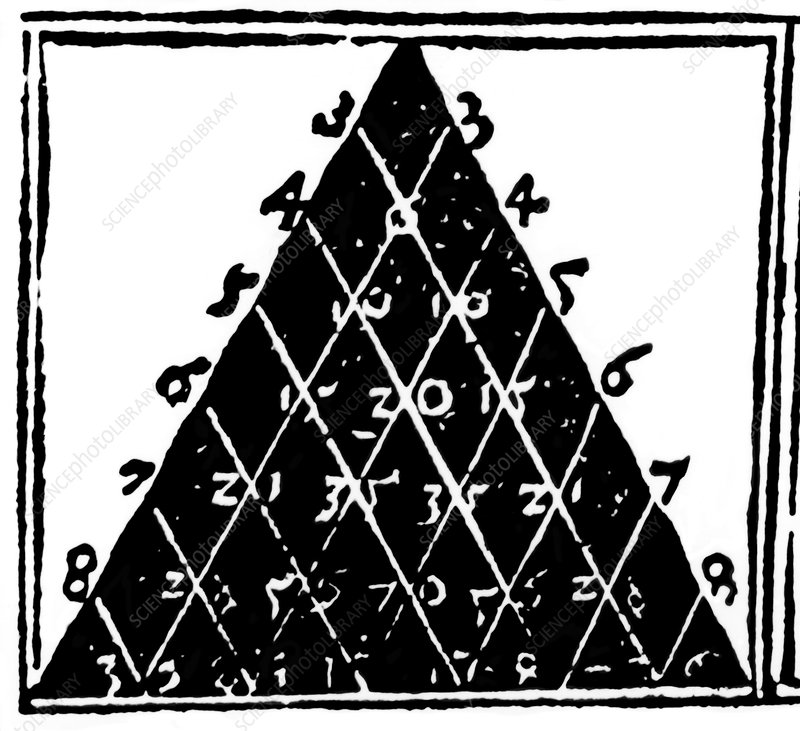
\includegraphics[width=0.5\textwidth]{Essay/Draft_2/Apianus.jpg}
\caption{Appearing on the title page of Kauffmans Rechnung (Ingolstadt, 1527) \citep{boyer1950}.}
\label{fig:apianus}
\end{figure}

\subsection{Historical Background}

Petrus Apianus (1495–1552), a German astronomer and mathematician, integrated the arithmetic triangle into his 1527 almanac \textit{Practica auf Deutsch} to simplify the calculation of Easter dates. Apianus’s algorithm exemplifies pragmatic Renaissance mathematics, prioritizing usability over precision. While its approximations limited long-term accuracy, the method’s design—rooted in the arithmetic triangle—showcased early modern efforts to systematize celestial computations. Its historical value lies not in precision but in democratizing astronomy, bridging medieval scholarship and the Scientific Revolution. Apianus’s printed triangle (Figure \ref{fig:apianus}) catered to Europe’s literate middle class, blending astronomy with print culture\citep{boyer1950}. 

\section{Tartaglia’s Combinatorial Probability}

\begin{figure}[h!tbp]
\centering
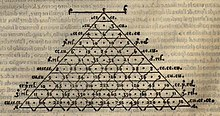
\includegraphics[width=0.3\textwidth]{Essay/Draft_2/Tartaglia.jpg}
\caption{Tartaglia’s probability tables \citep{tartaglia1556}.}
\label{fig:tartaglia}
\end{figure}

\subsection{Historical Background}

Niccolò Tartaglia (1500–1557), an Italian mathematician of the Renaissance era, pioneered combinatorial probability in his General Trattato di Numeri et Misure (1556). His work linked the arithmetic triangle to dice probabilities, reflecting Europe’s burgeoning interest in risk quantification for commerce and games of chance \citep{tartaglia1556}. Tartaglia’s tables (Figure \ref{fig:tartaglia}) quantified risk for gamblers, reflecting Renaissance Europe’s market-driven ethos \citep{hinz1992}.

\subsection{Mathematical Statement}

Tartaglia tried to use the table to calculate the probability of rolling a sum of 7 with two six-sided dice.

\subsection{Tartaglia's Method Using the Arithmetic Triangle}
\subsubsection{Step 1: Total Outcomes}
Two dice yield:
\[
6 \times 6 = 36 \text{ total outcomes}.
\]

\subsubsection{Step 2: Favorable Outcomes}
Tartaglia used the second row of the arithmetic triangle (1, 2, 1) to count combinations, later corrected to:
\[
\begin{array}{cccccccccccc}
\text{Sum} & 2 & 3 & 4 & 5 & 6 & 7 & 8 & 9 & 10 & 11 & 12 \\
\text{Ways} & 1 & 2 & 3 & 4 & 5 & 6 & 5 & 4 & 3 & 2 & 1 \\
\end{array}
\]
For sum \(7\), there are 6 favorable outcomes: \((1,6), (2,5), (3,4), (4,3), (5,2), (6,1)\) \citep{hald1990}.

\subsubsection{Step 3: Probability Calculation}
\[
P(\text{sum } 7) = \frac{\text{Favorable}}{\text{Total}} = \frac{6}{36} = \frac{1}{6}.
\]

\subsection{Mathematical Breakdown}

For Tartaglia's usage of the second row :\((1,2,1)\), it is limited since it is only applicable for binary outcomes. For the six-sided dice, either the triangle needs to be modified or generating function is required:

\subsubsection{Generating Function Approach}
The number of ways to roll sum \(k\) with \(n\) dice is the coefficient of \(x^k\) in:
\[
(x + x^2 + \cdots + x^6)^n.
\]
For \(n = 2\), the coefficient of \(x^7\) is 6 \citep{pascal1654}.

\subsubsection{Modern Generalization}
For \(n\) dice, the number of ways to roll sum \(k\) is:
\[
\binom{k - 1}{n - 1} - \text{adjustments for dice faces}.
\]

\subsubsection{Modified Triangle}

The modified triangle, the entries are derived from the generating function $(x+x^2+x^3+x^4+x^5+x^6)^2$ :

\begin{align*}
    n=1:& \text{1 1 1 1 1 1}\\
n=2:& \text{1 2 3 4 5 6 5 4 3 2 1}\\
n=3:& \text{1 3 6 10 15 21 25 27 27 25 21 15 10 6 3 1}\\
\end{align*}

Note that it also have the same symmetry property as the arithmetic triangle, also there is a recursive rule for the modified triangle:

\[
\text{Num}(k,n)=\sum^{6}_{i=1}\text{Num}(k-i,n-1)
\]

This shared some similarities with the recursive rule for arithmetic triangle:

\[
\binom{n}{k}=\binom{n-1}{k-1}+\binom{n-1}{k}
\]

\subsection{Error Analysis}
\begin{itemize}
\item \textbf{Initial Limitations}: Tartaglia's incomplete triangle undercounted sums (e.g., sum 4 as 1 vs. actual 3) \citep{tartaglia1556}.
\item \textbf{Refinements}: Pascal and Fermat expanded the triangle and formalized expectation theory \citep{pascal1654}.
\end{itemize}

\section{Conclusion}

Jia Xian’s iterative root extraction and Yang Hui’s refinements exemplify the triangle’s algebraic utility in governance, while Apianus’s lunar computations and Tartaglia’s probability tables highlight its combinatorial adaptability to Europe’s commercial and scientific demands. Strikingly, methods like Jia Xian’s approximation for cubic roots align with modern numerical techniques such as the Newton-Raphson method, underscoring the timelessness of these innovations. Yet their applications diverged profoundly, reflecting cultural imperatives: precision in statecraft versus probabilistic risk assessment in emerging markets. This duality not only enriches our understanding of mathematical history but also dismantles narratives of unilateral progress.

\newpage

\bibliographystyle{plainnat}
\bibliography{reference}

\newpage

\section{Reflection}

I think the Tartaglia part needs some more details. And perhaps some comparison with Chinese and European? I think there should be some connections between different sections, but some relations are included in the introduction and conclusion sections. Perhaps the math content is not that much?
\end{document}